\documentclass{article}
\usepackage[utf8]{inputenc}
\usepackage{graphicx}
\usepackage{amsmath}
\usepackage{amssymb}
\usepackage{mathrsfs}
\usepackage{pgfplots}
\usepackage[many]{tcolorbox}
\usepackage[margin = 0.5in]{geometry}
\usepackage{collectbox}

\usetikzlibrary{decorations.markings}
\tikzset{
    arrow inside/.style = {
        postaction = {
            decorate,
            decoration={
                markings,
                mark=at position #1 with {\arrow{>}}
            }
        }
    },
    arrow inside/.default = 0.5
}

\linespread{1.8}

\makeatletter
\newcommand{\mybox}{%
    \collectbox{%
        \setlength{\fboxsep}{1pt}%
        \fbox{\BOXCONTENT}%
    }%
}
\makeatother
\title{MAT 527: HW V}
\begin{document}

%%
%% Title 
%%
\begin{center}
\hrulefill \\
\vspace{-0.7cm}
\hrulefill \\
\vspace{-0.3cm}

\begin{Large}
\textbf{MAT 527:  Functions of a Complex Variable I} \\
\textbf{Homework V} \\
\end{Large}
\begin{large}
\end{large}
\vspace{-7mm}
\noindent \textbf{Date:} \hfill \textbf{Author:}\\
\noindent\today \hfill Nolan R. H. Gagnon \\

\vspace{-0.4cm}
\hrulefill \\
\vspace{-0.7cm}
\hrulefill
\end{center}

\vspace{7mm}

%%
%% PROBLEM ONE
%%
\noindent\mybox{\textbf{Problem 1}}  Compute the improper integral $$\int\limits_0^{\infty}\frac{\sin x}{x} \hspace{1mm} dx$$ \textbf{(a)} using Cauchy's Theorem and \textbf{(b)} using Cauchy's Integral Formula.

\vspace{5mm}

\noindent\mybox{\textbf{Solution}}  First note that $\sin(x) = \text{Im}\left(e^{ix}\right)$.  Thus, 
\begin{align}
\int\limits_0^{\infty}\frac{\sin x}{x} \hspace{1mm} dx &= \text{Im}\left(\int\limits_0^{\infty}\frac{e^{ix}}{x} \hspace{1mm} dx\right).
\end{align}

\noindent To compute the integral on the right-hand side of $(1)$, first let $f(z) = \frac{e^{iz}}{z}$, which is holomorphic everywhere except at $z=0$ (since it is a ratio of entire functions).  Next, define $\mathscr{C}$ as the closed, simple contour given in the figure below: 

\vspace{7mm}

\begin{center}
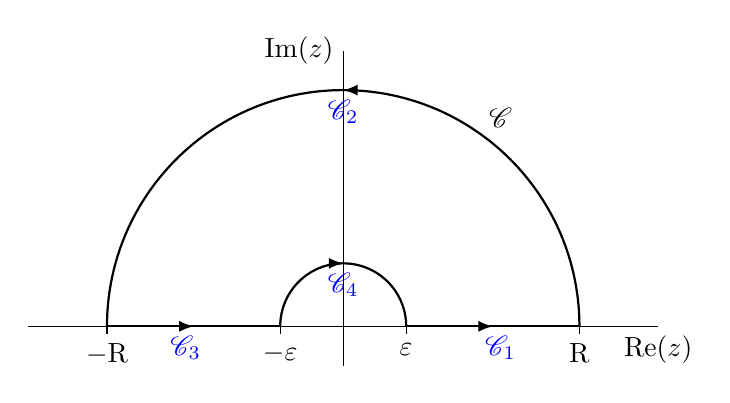
\begin{tikzpicture}[>=latex]
    \begin{scope}[xshift=15cm]
        % Axes
        \draw
            (-4,0) -- (4,0) node[below] {$\text{Re}(z)$}
            (0,-0.5) -- (0,3.5) node[left] {$\text{Im}(z)$};
            
        % R Ticks
        \draw (3, 0) -- (3, -0.1) node[below] {$\mathrm{R}$}
            (-3, 0) -- (-3, -0.1) node[below] {$-\mathrm{R}$};
            
        % epsilon ticks
        \draw (0.8, 0) -- (0.8, -0.1) node[below] {$\varepsilon$}
        	  (-0.8, 0) -- (-0.8, -0.1) node[below] {$-\varepsilon$};
        
        % Contour
        \draw[arrow inside, thick] (3,0) --
            (3, 0) node[above left] {}
            arc[start angle=0, end angle=180, radius=3]
            (-3, 0) node[above right] {} --
            (-3, 0);
            
        \draw (2, 2.4) node[above] {$\mathscr{C}$};  
         
        \draw[arrow inside, thick] (0.8, 0) -- (3, 0);
        
        \draw[arrow inside, thick] (-3,0) -- (-0.8, 0);
        
        \draw[arrow inside, thick]
        (-0.8, 0) arc[start angle=180, end angle=0, radius=0.8];
        
        % Label subsections of the contour
        \draw (2,0) node[below] {\textcolor{blue}{$\mathscr{C}_1$}};
        \draw (0,3) node[below] {\textcolor{blue}{$\mathscr{C}_2$}};
        \draw (-2,0) node[below] {\textcolor{blue}{$\mathscr{C}_3$}};
        \draw (0, 0.8) node[below] {\textcolor{blue}{$\mathscr{C}_4$}};
        
    \end{scope}
\end{tikzpicture}
\end{center}

\vspace{7mm}

\noindent Since $\mathscr{C}$ does not contain $z=0$, our function $f(z)$ is holomorphic in and on $\mathscr{C}$.  Therefore 
\begin{align}
\int\limits_{\mathscr{C}} f(z) \hspace{1mm} dz &= 0,
\end{align}

\noindent by Cauchy's Theorem.  The integral in $(2)$, however, can be considered as the sum of four integrals along the four sections of the contour $\mathscr{C}$ (i.e., $\mathscr{C}_1$, $\mathscr{C}_2$, $\mathscr{C}_3$, and $\mathscr{C}_4$).  The integrals along $\mathscr{C}_1$ and $\mathscr{C}_2$ will become real integrals, while the integrals along $\mathscr{C}_2$ and $\mathscr{C}_4$ will need to be parameterized.  The contour $\mathscr{C}_2$ can be parameterized by letting $z=Re^{it}$ and letting $t$ range from $0$ to $\pi$, whereas $\mathscr{C}_4$ can be parameterized by letting $z=\varepsilon e^{it}$ and letting $t$ range from $\pi$ to $0$. Hence,    

\begin{align}
\int\limits_{\mathscr{C}} f(z) \hspace{1mm} dz &= \int\limits_{\mathscr{C}_1} f(z) \hspace{1mm} dz + \int\limits_{\mathscr{C}_2} f(z) \hspace{1mm} dz +
\int\limits_{\mathscr{C}_3} f(z) \hspace{1mm} dz +
\int\limits_{\mathscr{C}_4} f(z) \hspace{1mm} dz \\
&= \int\limits_{\varepsilon}^R\frac{e^{ix}}{x} \hspace{1mm} dx + \int\limits_0^\pi f\left(Re^{it}\right)Rie^{it}\hspace{1mm} dt + 
\int\limits_{-R}^{-\varepsilon} \frac{e^{ix}}{x} \hspace{1mm} dx +
\int\limits_\pi^0 f\left(\varepsilon e^{it}\right)\varepsilon ie^{it}\hspace{1mm} dt \\
&= \int\limits_{\varepsilon}^{R}\frac{e^{ix}}{x} \hspace{1mm} dx + \int\limits_{\varepsilon}^R \frac{e^{-ix}}{-x} \hspace{1mm} dx + \int\limits_0^\pi \frac{e^{iRe^{it}}}{Re^{it}}Rie^{it} \hspace{1mm} dt + \int\limits_\pi^0 \frac{e^{i\varepsilon e^{it}}}{\varepsilon e^{it}} \varepsilon ie^{it} \hspace{1mm} dt \\
&= \int\limits_{\varepsilon}^R \frac{e^{ix} - e^{-ix}}{x} \hspace{1mm} dx + i\int\limits_0^\pi e^{iRe^{it}} \hspace{1mm} dt - i\int\limits_0^\pi e^{i\varepsilon e^{it}} \hspace{1mm} dt \\
&= 0.
\end{align}

\noindent It can be shown that the second integral in $(6)$ converges to $0$ as $R$ tends to infinity.  Note that 
\begin{align}
\left| \int\limits_0^\pi e^{iRe^{it}} \hspace{1mm} dt\right| &= \left| \int\limits_0^\pi e^{iR\cos t}e^{-R\sin t} \hspace{1mm} dt\right| \\
&\leq \int\limits_0^\pi \left| e^{iR\cos t}\right|\left|e^{-R\sin t} \right| \hspace{1mm} dt \\
&= \int\limits_0^\pi e^{-R\sin t} \hspace{1mm} dt \\
&= 2\int\limits_0^{\frac{\pi}{2}} e^{-R\sin t} \hspace{1mm} dt.
\end{align}

\noindent Now consider the function $g(t) = \frac{2R}{\pi}t$.  Note that $g(0) = 0 = R\sin(0)$ and $g\left(\frac{\pi}{2}\right) = R = R\sin\left(\frac{\pi}{2}\right)$.  This, along with the fact that $\sin t$ is continuous and concave down on the interval $\left(0,\frac{\pi}{2}\right]$, means that $R\sin t \geq \frac{2R}{\pi}t$ on $\left[0,\frac{\pi}{2}\right]$.  Thus, $e^{-\frac{2R}{\pi}t} \geq e^{-R\sin t}$ on $\left[0, \frac{\pi}{2}\right]$.  Therefore,
\begin{align}
2\int\limits_0^{\frac{\pi}{2}} e^{-R\sin t} \hspace{1mm} dt &\leq 2\int\limits_0^{\frac{\pi}{2}} e^{-\frac{2R}{\pi}t} \hspace{1mm} dt \\
&= \left[\frac{-2\pi}{2R}e^{-\frac{2R}{\pi}t}\right]^{\frac{\pi}{2}}_0 \\
&= \frac{\pi}{R}\left[1-e^{-R}\right],
\end{align}

\noindent which tends to $0$ as $R$ tends to infinity.  Thus, it must also be true that $\int\limits_0^\pi e^{iRe^{it}} \hspace{1mm} dt \longrightarrow 0$ as $R\rightarrow \infty$.  This means that $(6)$ can now be rewritten as 
\begin{align}
\int\limits_{\varepsilon}^{\infty} \frac{e^{ix} - e^{-ix}}{x} \hspace{1mm} dx &= i\int\limits_0^{\pi}e^{i\varepsilon e^{it}} \hspace{1mm} dt.
\end{align}

\noindent We can rewrite the right-hand side of $(15)$ using a Maclaurin series.  That is $$e^{i\varepsilon e^{it}} = 1 + i\varepsilon e^{it} + \mathscr{E}\left(i\varepsilon e^{it}\right)i \varepsilon e^{it},$$ where $\mathscr{E}(w)$ tends to $0$ as $w$ tends to $0$.  Therefore,
\begin{align}
\int\limits_{\varepsilon}^{\infty} \frac{e^{ix} - e^{-ix}}{x} \hspace{1mm} dx &= i\int\limits_0^\pi 1 \hspace{1mm} dt - \int\limits_0^\pi \varepsilon e^{it} \hspace{1mm} dt - \int\limits_0^\pi \mathscr{E}\left(i\varepsilon e^{it}\right) \varepsilon e^{it} \hspace{1mm} dt \\
&= i\pi - \int\limits_0^\pi \varepsilon e^{it} \hspace{1mm} dt - \int\limits_0^\pi \mathscr{E}\left(i\varepsilon e^{it}\right) \varepsilon e^{it} \hspace{1mm} dt.
\end{align}

\noindent We now show that the two integrals in $(17)$ tend to $0$ as $\varepsilon \rightarrow 0^{+}$.  First, let $a>0$.  Choose $\delta = \frac{a}{\pi}$.  Then whenever $0<\varepsilon<\frac{a}{\pi}$, we have
\begin{align}
\left| \int\limits_0^\pi \varepsilon e^{it} \hspace{1mm} dt - 0\right| &\leq \int\limits_0^\pi \left| \varepsilon e^{it} \right| \hspace{1mm} dt \\
&= \int\limits_0^\pi\varepsilon \hspace{1mm} dt \\
&= \varepsilon \pi \\
&<\frac{a}{\pi} \pi \\
&= a.
\end{align}

\noindent Therefore, $\int\limits_0^\pi \varepsilon e^{it} \hspace{1mm} dt \longrightarrow 0$ as $\varepsilon \rightarrow 0^+$.   
\end{document}
